\documentclass[10pt]{article}
\usepackage{icmlko}

\icmlmeta{IP 파운데이션 월드모델}{318}{몫이 없으면 삼켜진다}{아이돌이 풀링에서 왜 죽는지 갈랐다 --- 청력은 되는데 들을 이유가 없다}

\begin{document}

\twocolumn[
\icmlheader

\begin{abstract}
노트 317이 아이돌을 ``풀링이 죽이는 유일한 자리''로 냈다 --- 혼자 0.5977
인데 풀에 넣으면 0.1012($t{=}{-}2.01$). 갈랐다. \textbf{제 행은 쓰인다} ---
아이돌의 학습 라벨을 풀에서 지우면 0.1012 $\to$ 0.0125 로 더 떨어진다.
그런데 아이돌은 학습 풀의 \textbf{0.52\%}(54/10,393)다. \textbf{청력은
되는데}(54행 $>$ F18 문턱 22, 노트 281) \textbf{들을 이유가 없다} --- 0.5\%를
위한 분할이 탐욕 기준을 못 이긴다. 시험했다: 풀을 \textbf{작은 도메인부터}
하나씩 키우며 아이돌을 봤다. \textbf{몫이 줄수록 단조롭게 무너진다} ---
100\% 0.598 · 36\% \textbf{0.639} · 21.5\% 0.541 · 10.6\% 0.481 · 6.5\%
0.500 · \textbf{2.35\% 0.286} · 0.96\% 0.240 · 0.52\% \textbf{0.101}.
풀 크기(log)와의 스피어만이 \textbf{$-$0.943}($p{<}$1e-4)이고
\textbf{6.5\%와 2.35\% 사이에 절벽}이 있다. 그리고 \textbf{작은 풀에서는
오히려 오른다} --- 도서와 둘이면(몫 36\%) 0.6391 로 혼자보다 낫다.
다른 도메인을 같은 그림에 놓으면 법칙이 보인다: \textbf{몫이 1\% 아래인
셋만 크게 갈리고}(도서 $+$0.28 · 시장팝업 $+$0.25 · 아이돌 $-$0.50)
\textbf{10\% 위인 넷은 $\pm$0.03 이다.} \textbf{몫이 크기를 정하고 솔로
적합의 질이 방향을 정한다.}
\end{abstract}
]

\section{제 행은 쓰인다}

노트 317이 남긴 첫 갈래가 ``아이돌은 왜 죽나''였다. 네 갈래를 놓고 쟀다.

\begin{center}\footnotesize
\begin{tabular}{lr}
\hline
아이돌 유보 $\rho$ & \\
\hline
혼자 적합 & \textbf{0.5977} \\
풀링 (아이돌 학습 포함) & 0.1012 \\
풀링 (아이돌 학습도 뺌) & \textbf{0.0125} \\
\hline
\end{tabular}
\end{center}

\textbf{제 행이 쓰이긴 한다}(0.0125 $\to$ 0.1012, $+$0.089). 묻혀서 안 쓰이는
게 아니라 \textbf{쓰이는데도 모자란} 것이다.

\paragraph{다른 갈래는 약하다} 라벨 척도는 특별하지 않고(중앙 5.071 · IQR
0.922 --- 웹툰 4.742/0.667 과 비슷하며 \texttt{pooled} 은 도메인 안 순위를
쓴다). 축 프로파일 상관은 남과 $-$0.23 $\sim$ $+$0.54 로 약하지만 그것만으로
0.50 을 못 설명한다. \textbf{남은 것은 무게다} --- 54/10,393 ${=}$ 0.52\%.

\paragraph{청력은 되는데} 노트 281의 청력 문턱은 F18 에서 22행이고 아이돌은
54행이다. \textbf{도메인 전용 분할을 만들 \emph{수}는 있다.} 그런데 분할
선택은 10,393행 전체의 이득으로 정해진다 --- \textbf{0.5\%를 위한 분할이
이길 일이 없다.} \textbf{청력은 필요조건이고 무게가 충분조건이다.}

\section{몫을 훑었다}

\begin{figure*}[t]
\centering
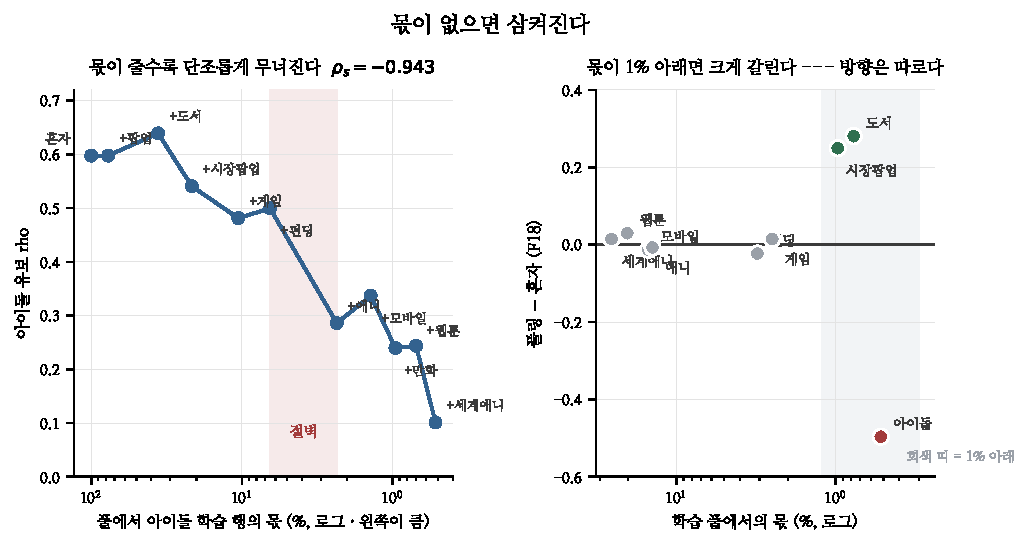
\includegraphics[width=\textwidth]{figs/share.pdf}
\caption{왼쪽 --- 풀을 작은 도메인부터 키우며 잰 아이돌 유보 $\rho$.
오른쪽 --- 다른 도메인들의 몫과 풀링 이득.}
\end{figure*}

\begin{center}\footnotesize
\begin{tabular}{lrrr}
\hline
풀 & 학습 & 아이돌 몫 & 아이돌 $\rho$ \\
\hline
혼자 & 54 & 100.0\% & 0.5977 \\
$+$팝업 & 70 & 77.1\% & 0.5977 \\
$+$도서 & 150 & 36.0\% & \textbf{0.6391} \\
$+$시장팝업 & 251 & 21.5\% & 0.5407 \\
$+$게임 & 510 & 10.6\% & 0.4813 \\
$+$펀딩 & 830 & 6.5\% & 0.4995 \\
\hline
$+$애니 & 2,297 & 2.35\% & \textbf{0.2860} \\
$+$모바일 & 3,856 & 1.40\% & 0.3368 \\
$+$만화 & 5,639 & 0.96\% & 0.2398 \\
$+$웹툰 & 7,745 & 0.70\% & 0.2436 \\
$+$세계애니 & 10,393 & 0.52\% & \textbf{0.1012} \\
\hline
\end{tabular}
\end{center}

\textbf{단조롭다} --- 풀 크기(log)와의 스피어만 \textbf{$-$0.943}
($p{<}$1e-4). 그리고 \textbf{6.5\%와 2.35\% 사이에 절벽이 있다}: 위쪽은
0.48$\sim$0.64, 아래쪽은 0.10$\sim$0.34.

\paragraph{작은 풀은 오히려 돕는다} 아이돌 $+$ 도서(둘 다 얇다, 몫 36\%)가
\textbf{0.6391 로 혼자(0.5977)보다 낫다.} \textbf{풀링이 나쁜 게 아니라
\emph{무게가 안 맞는} 풀링이 나쁘다.}

\section{다른 도메인도 같은 그림에 있다}

\begin{center}\footnotesize
\begin{tabular}{lrr}
\hline
도메인 & 학습 몫 & 풀링 $-$ 혼자 \\
\hline
세계애니 & 25.5\% & $+$0.015 \\
웹툰 & 20.3\% & $+$0.030 \\
모바일 & 15.0\% & $-$0.013 \\
애니 & 14.1\% & $-$0.007 \\
펀딩 & 3.1\% & $-$0.023 \\
게임 & 2.5\% & $+$0.015 \\
\hline
시장팝업 & \textbf{0.97\%} & \textbf{$+$0.249} \\
도서 & \textbf{0.77\%} & \textbf{$+$0.281} \\
아이돌 & \textbf{0.52\%} & \textbf{$-$0.496} \\
\hline
\end{tabular}
\end{center}

\textbf{1\% 아래인 셋만 크게 갈린다.} 10\% 위인 넷은 전부 $\pm$0.03 이다.

\begin{center}\small
\begin{tabular}{ll}
\hline
\textbf{몫} & 풀링 효과의 \textbf{크기}를 정한다 \\
\textbf{솔로 적합의 질} & 풀링 효과의 \textbf{방향}을 정한다 \\
\hline
\end{tabular}
\end{center}

몫이 1\% 아래면 그 도메인은 \textbf{풀이 시키는 대로} 한다. 제 솔로 적합이
나빴으면 이득이고(도서 0.109 $\to$ 0.390 · 시장팝업 0.161 $\to$ 0.410)
좋았으면 손해다(아이돌 0.598 $\to$ 0.101).

\section{그래서 무엇을 할 수 있나}

\begin{center}\footnotesize
\begin{tabular}{ll}
\hline
지금 할 수 있는 것 & \\
\hline
얇은 도메인끼리 따로 풀 & 아이돌 $+$ 도서가 둘 다 낫다 \\
표본 가중 & 몫을 인위로 올린다 --- 안 해 봤다 \\
도메인 전용 축 & 분할이 져도 값은 산다(노트 309) \\
\hline
안 되는 것 & \\
\hline
그냥 다 넣기 & 아이돌이 $-$0.50 을 낸다 \\
\hline
\end{tabular}
\end{center}

\textbf{``파운데이션이니까 다 넣는다''가 틀렸다.} 이 판에서 다 넣는 것은
얇은 셋 중 둘을 살리고 하나를 죽인다. \textbf{누구와 묶느냐가 넣느냐 마느냐
보다 중요하다.}

\paragraph{남은 것}
\begin{center}\small
\begin{tabular}{ll}
\hline
갈래 & 왜 \\
\hline
표본 가중을 걸면 & 몫을 올리는 직접적인 손잡이 \\
얇은 것끼리 풀 & 아이돌·도서·시장팝업·팝업 넷 \\
절벽이 5\% 인가 & 도메인마다 다른가 \\
선형에도 절벽이 있나 & F6 은 탐욕 분할이 없다 \\
\hline
\end{tabular}
\end{center}

\paragraph{규약} \textbf{``들을 수 있나''와 ``들을 이유가 있나''는 다르다.}
노트 281이 청력 문턱을 잰 뒤로 이 실험실은 ``문턱을 넘으면 배운다''로
읽어 왔다. 아이돌은 문턱의 두 배 반(54 대 22)인데 안 배운다 --- \textbf{탐욕
분할은 전체 이득으로 고르므로 몫이 없으면 후보에 올라도 안 뽑힌다.}
그리고 \textbf{용량 곡선을 그려라} --- ``풀링이 해롭다''는 관측이었는데
몫을 훑으니 $\rho_s{=}{-}0.943$ 짜리 법칙이 나왔고 \textbf{절벽 위치까지
보인다.}

\end{document}
